\documentclass[tikz]{standalone}
\usepackage{ctex}
\usepackage{tikz}
\usepackage{pgfplots}
\pgfplotsset{compat=1.18}   % 使用较新版本语法
\usetikzlibrary{positioning, arrows.meta, intersections, calc, fit, backgrounds}
\usepgfplotslibrary{fillbetween}  % 用于填充区域
\begin{document}

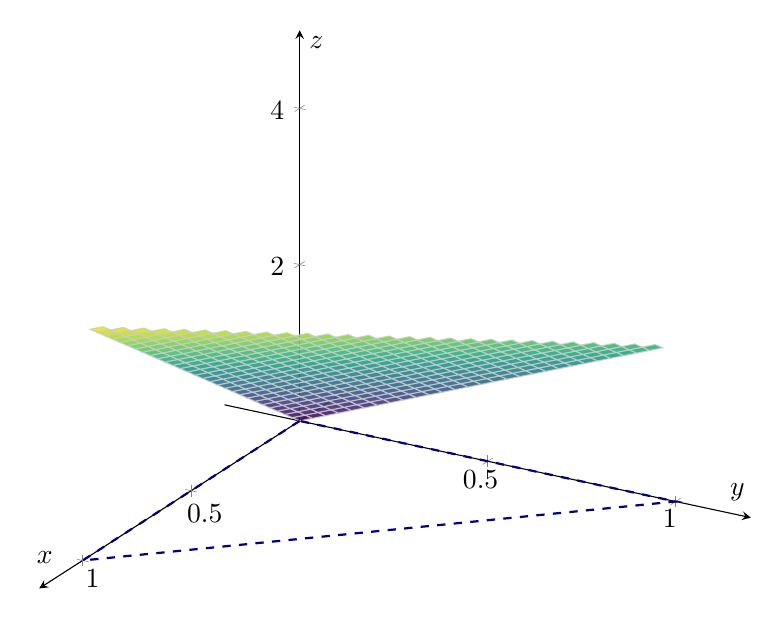
\begin{tikzpicture}
        \begin{axis}[
                view={120}{30},
                axis lines=center,
                xlabel={$x$}, ylabel={$y$}, zlabel={$z$},
                xtick={0,0.5,1}, ytick={0,0.5,1}, ztick={0,2,4},
                width=\textwidth,
                xmin=-0.2, xmax=1.2,
                ymin=-0.2, ymax=1.2,
                zmin=0, zmax=5,
                colormap/viridis,
                samples=30,
                clip=false
            ]

            % 绘制曲面 z = 3x + 2y，定义域为三角形 0<=x<=1, 0<=y<=1-x
            \addplot3[
                surf,
                domain=0:1,
                domain y=0:1,
                restrict expr to domain={y+x}{0:1},  % 关键：限制 y 的上限为 1-x
                opacity=0.85,
                faceted color=black!20,
                fill opacity=0.9
            ] ({x}, {y}, {3*x + 2*y});

            % 绘制底面三角形（虚线）
            \draw[thick, dashed, blue!50!black]
            (axis cs:0,0,0) -- (axis cs:1,0,0) -- (axis cs:0,1,0) -- cycle;
        \end{axis}
    \end{tikzpicture}
\end{document}